\documentclass[dvips,12pt]{article}

\usepackage[pdftex]{graphicx}
\usepackage{subcaption}
\usepackage{float}
\usepackage{url}
\usepackage[utf8]{inputenc}
\usepackage{geometry}
\usepackage{setspace}
\usepackage{amsmath}
\usepackage{txfonts}

% From amsmath, prepend equation numbers with section number
%\numberwithin{equation}{section}

% graphicx: Where should graphics be found?
\graphicspath{ {figures/} }
\graphicspath{{./figures/}} % allows figures to be placed in a different folder

% Setup margins and paper size
\geometry{
  letterpaper,
  total={170mm,257mm},
  left=20mm,
  top=20mm,
  bottom=25mm
}

%\title{ECEN 773 Project: Planar VTOL}
%\author{Jesse Wynn}
%\date{April 20, 2017}

\begin{document}

\begin{titlepage}

\begin{center}

\vspace*{\fill}

\vspace{0.5in}

% Insert your title here
{ \LARGE \bfseries LQR Control of a Planar VTOL}\\[.25in]

\large
by\\[.25 in]
% Change your name here
Jesse S. Wynn\\[1in]

Final Project for ECEN 773 (Linear Systems Theory) \\
Brigham Young University \\

\vspace{1in}

\today

\vspace*{\fill}

\end{center}

\end{titlepage}

\section{Introduction}
For this project I wanted to implement an LQR controller on a simple MIMO linear system.  The dynamic system I chose to model and control was a simple two-dimensional UAV, or planar VTOL.  The planar VTOL seemed to be an ideal system to study since it is relatively simple, yet it has many similarities to more complex rotor-craft systems such as quadrotor UAVs.  In Dr. Beards undergraduate controls class, we used the planar VTOL as an ongoing case-study exercise, and this project is an extension of that work.  The specifics of this project include re-modeling the linear state-space system, and then implementing LQR control, set-point control, and observer-based control in MATLAB and SIMULINK.  

\section{Linear Dynamic Model}

The planar VTOL is characterized by a point mass $m_c$ at the vehicle center, and two additional point masses $m_l$ and $m_r$ at a distance $d$ on opposite sides of the vehicle.  The term $m_c$ represents the vehicle's main body and electronics, and $m_l$ and $m_r$ represent electric motors and propellers.  There are three forces acting on the VTOL which are $f_l$, $f_r$, and then the force of gravity $f_g$.  The vehicle pose is defined by horizontal displacement $z$, angle $\theta$, and vertical displacement $h$. An illustration is given below.

\begin{figure}[h] %  figure placement: here, top,  bottom, or page
   \centering
   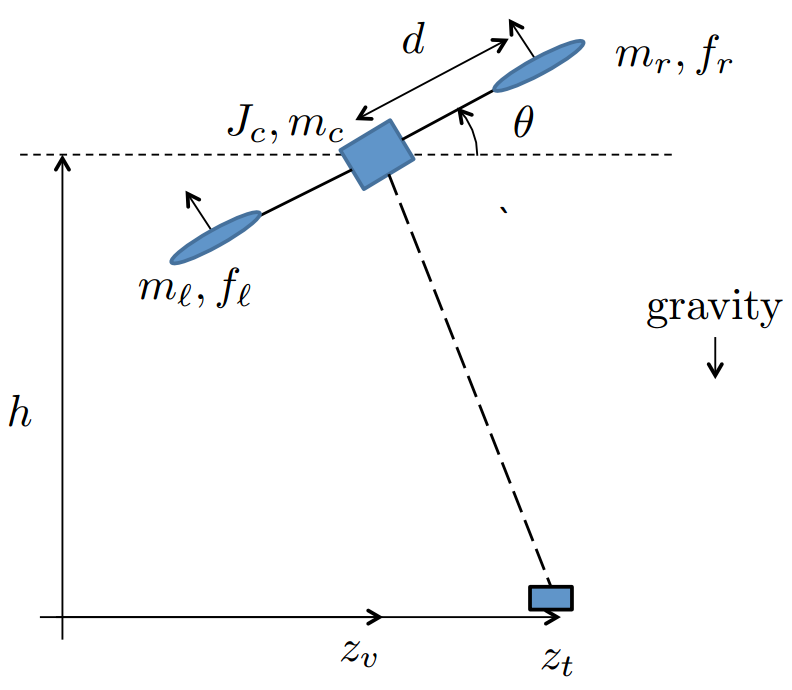
\includegraphics[trim = 0mm 0mm 0mm 0mm,clip,width=3in]{planar_vtol.png}
   \caption{Planar VTOL physical System Definition}
   \label{fig:vtol}
\end{figure}

The dynamic model (or plant) that is used in simulation includes the full non-linear dynamics of the VTOL.  For the controls design however, a much simpler linear model is used. Using principles of linearization from the textbook, the linear dynamics of the system were found to be

\begin{equation}
\ddot{z} = \frac{-F_e}{m_c + 2m_r}  + \frac{-\mu\dot{z}}{m_c + 2m_r}
\end{equation}

\begin{equation}
\ddot{\theta} = \frac{\tau}{J_c + 2m_r d^2}
\end{equation}

\begin{equation}
\ddot{h} = \frac{\tilde{F}}{m_c + 2m_r}
\end{equation}

where $F_e$ is an equilibrium force to counteract gravity, $\mu$ is a damping force to represent the propeller drag, $J_c$ is the VTOL's rotational moment of inertia, and $\tau$ and $\tilde{F}$ capture the combined force and torque from $f_l$ and $f_r$. These linear dynamics can be put into state-space form as follows:



\begin{gather}
 \dot{x}
 =
 \begin{bmatrix}
     \dot{z} \\
     \dot{\theta} \\
     \dot{h} \\
     \ddot{z} \\
     \ddot{\theta} \\
     \ddot{h} \\
   \end{bmatrix}
   =   
   \begin{bmatrix}
        0 & 0 & 0 & 1 & 0 & 0  \\
        0 & 0 & 0 & 0 & 1 & 0 \\
        0 & 0 & 0 & 0 & 0 & 1 \\
        0 & \frac{-F_e}{m_c + 2m_r} & 0 & 0 & 0 & 0 \\
        0 & 0 & 0 & 1 & 0 & 0 \\
        0 & 0 & 0 & 1 & 0 & 0 \\
      \end{bmatrix}
\end{gather}

\section{Full-State Feedback LQR}

\section{Set-Point LQR Controller}

\section{Implementing an Observer}



\end{document}